\section{Itération 2: ( 3/8/2017 - 3/28/2017 )}

\subsection{L'objectif du sprint}
La méthodologie Scrum a eu un impact positif sur les développeurs, du point de vue social, elle
a valorisé le travail en équipe, la solidarité, le respect et la communication entre toutes les
parties prenantes (client, développeurs...). Elle a aussi changé leur vison sur le développement
des logiciels.\\
L'objectif de cette itération est d'ajouter un système de gestion des rapport et d'améliorer
la qualité de gestion de la page ``Dashboard''.
  \subsubsection{Planification de l'itération 2}
  Au cous de la réunion de planification nous avons sélectionné les tâches à réaliser au
  cours de cette itération tout en accord avec le ”Product-Owner”.
  \subsubsection{Préparation de la liste des tâches}
 \begin{center}
    \footnotesize
    \begin{longtable}{| p{1cm} | p{5cm} | p{7cm} | p{1cm} |}
        \caption{Taches à faire de la première itération}
        \label{tab:sprint2-backlog} \\

 \hline
 \multicolumn{1}{|c}{\textbf{Réf}} &
 \multicolumn{1}{|c}{\textbf{Spécification}} &
 \multicolumn{1}{|c}{\textbf{Description}} &
 \multicolumn{1}{|c|}{\textbf{Priorité}} \\ \hline
 \endhead

 \hline \multicolumn{4}{|r|}{{Continué en page suivante$\dotsc$}} \\ \hline
 \endfoot

 \hline \hline
 \endlastfoot

\hline
1 & Recherche trajectoire & Notion de trajectoirec & 1 \\ \hline
2 & Affichage du trajet sur la carte&Trajectoire affichée sur la carte d'un ID  & 1 \\ \hline
3 &Réception des données des ralentisseur &Table qui contient les informations des ralentisseur & 1 \\ \hline
4&Responsive design& IHM adaptable & 2 \\ \hline
5 & Ajout un bouton ralentisseur &Enable,Disabled respecte l'IHM  & 2 \\ \hline
6 & Filtrage des marqueurs dans la carte & légende simplifier & 1 \\ \hline
7 & chargement de l'image & Image temporaire dans le serveur jusqu'à la validation & 1 \\ \hline
8 & Enregistrement des informations du rapport dans la BD rapport& Enregistrer les données lors de la validation ou suppression après time-out & 1 \\ \hline
9 & Recherche test unitaires & Comment simplifier le travail en utilisant le test unitaire cote serveur  & 1 \\ \hline
10 & Recherche framework PHP & & 2 \\ \hline 
11 &Groupement des secousse sur la carte & Regrouper les secousses lors d'un zoom out sur la carte & 3 \\ \hline
\end{longtable}
\end{center}

  \subsubsection{Estimation de la deuxième itération}
  Comme l'iteration précédant, Nous avons fixé la période de cette itération à 3 semaine
  \begin{table}[htbp]
    \centering
    \begin{tabular}{| c | c | c | c |}
\hline
\textbf{Membre} & \textbf{Nombre d'heures par jour} & \textbf{Nombre de jours présent} & \textbf{Total en heures} \\ \hline
\hline

Moez & 8 & 18& 144\\ \hline
Rihab & 8 & 18 & 144 \\ \hline
\multicolumn{2}{c|}{} & \textbf{Total} & 288 \\ \cline{3-4}
    \end{tabular}
    \caption{Nombre d'heures de travail estimé de l'itération 2}
    \label{tab:sprint2-capacity}
\end{table}
\begin{center}
    \begin{longtable}{| l | l | l |}
        \caption{Nombre d'heures estimé pour la réalisation des taches}
        \label{tab:sprint2-estimation} \\

 \hline
 \multicolumn{1}{|c}{\textbf{Spécification}} &
 \multicolumn{1}{|c}{\textbf{Membre}} &
 \multicolumn{1}{|c|}{\textbf{Heures}} \\ \hline
 \endhead

 \hline \multicolumn{3}{|r|}{{Continué en page suivante$\dotsc$}} \\ \hline
 \endfoot

 \hline \hline
 \endlastfoot

\hline
Recherche trajectoire & Rihab & 5 x 2 \\ \hline
Affichage du trajet sur la carte& Moez & 13 x 2 \\ \hline
Réception des données des ralentisseur& Moez & 5 \\ \hline
Responsive design & Rihab & 5 x 2 \\ \hline
Ajout un bouton ralentisseur& Rihab & 13 x 2 \\ \hline
 Filtrage des marqueurs dans la carte  & Rihab & 13 \\ \hline
chargement de l'image & Moez & 5 \\ \hline
Enregistrement des informations du rapport dans la BD rapport & Moez & 5 \\ \hline
 Recherche test unitaires & Moez & 5 \\ \hline
Recherche framework PHP & Moez & 5 \\ \hline
Groupement des secousse sur la carte  & Rihab & 5 \\ \hline
\end{longtable}
\end{center}
\subsection{Mises des normes}

Les critaires à respecter pour cette itération sont:

\begin{itemize}
        \item \HTODO{Qualité trajectoire}{en quentité et qualité}
        \item Architecture de back-end doit étre modulaire: On doit changer
            notre code procédurale par un code orienté objet et minimiser la
            duplication du code et séparer le code des models et le code des
            controlleurs.
        \item Affiche claire et responsive des marqueurs dans la carte meme si
            le nombre est trés élevé.
\end{itemize}

\paragraph{Qualité d trajectoire}

\paragraph{Qualité du code}

\paragraph{IHM Responsive}

\subsection{Modélisation UML}

\subsection{Évaluation suivant les normes mise}

\subsubsection{Produit de l'itération}

A la fin de l'itération 2,nous détaillons les différentes spécifications qui caractérisent et 
implémenté le systeme de gestion des rapport.
\paragraph{Page ``Rapport''}
Dans cette page, nous donne la main à l'utilisateur pour faire un petit rapport comme expliqué dans la
figure \ref{fig:sprint2-rapport-screenshot1} . 
\TODO{description comment l'envoi les information et comment l'enregister dans serveur }
\begin{figure}[htbp]
  \centering
  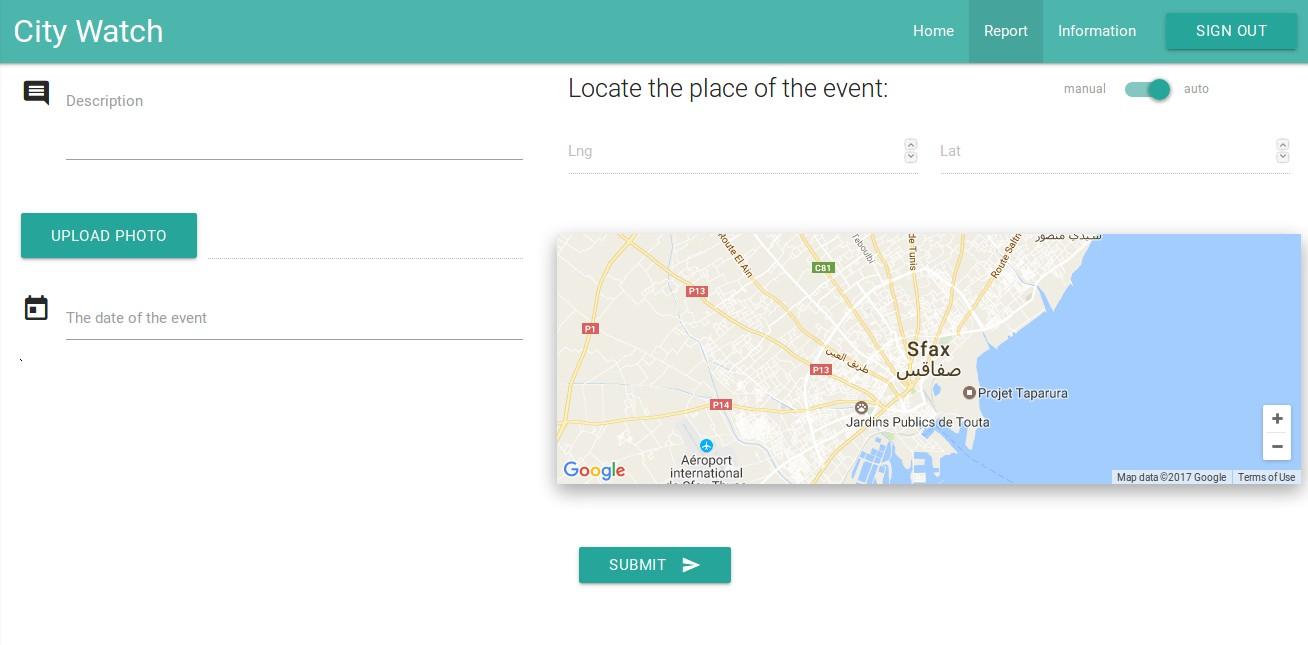
\includegraphics[width=0.7\textwidth]{sprint2-rapport-screenshot1}
  \caption{Page Rapport}
  \label{fig:sprint2-rapport-screenshot1}
\end{figure}
\paragraph{Page ``Dashboard''}
L'utilitaire de regroupement de marqueurs vous aide à gérer plusieurs marqueurs à différents niveaux de zoom.
Précisément, les  marqueurs  sont en fait des éléments à ce stade et ne deviennent réellement des
marqueurs qu'après leur rendu. Par souci de clarté, nous ne parlerons que de marqueurs 
dans ce document.

Lorsqu'un utilisateur affiche la carte à un niveau de zoom élevé comme montre la
figure~\ref{fig:sprint2-dashboard-screenshot1}, les différents marqueurs
s'affichent sur la carte. Lorsqu'il effectue un zoom arrière comme montre la
figure~\ref{fig:sprint2-dashboard-screenshot2}, les marqueurs se regroupent pour faciliter la consultation de la carte.

\begin{figure}[htbp]
    \begin{subfigure}{.5\textwidth}
    \centering
  \centering
  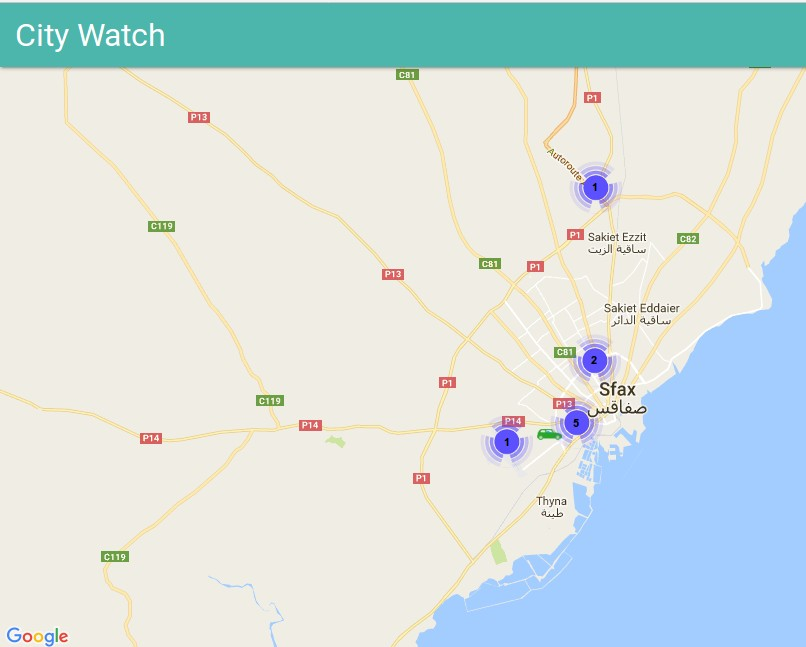
\includegraphics[width=.8\linewidth]{sprint2-dashboard-screenshot1}
  \caption{Groupement activé en un zoom bas}
  \label{fig:sprint2-dashboard-screenshot1}
\end{subfigure}
\begin{subfigure}{.5\textwidth}
    \centering
  \centering
  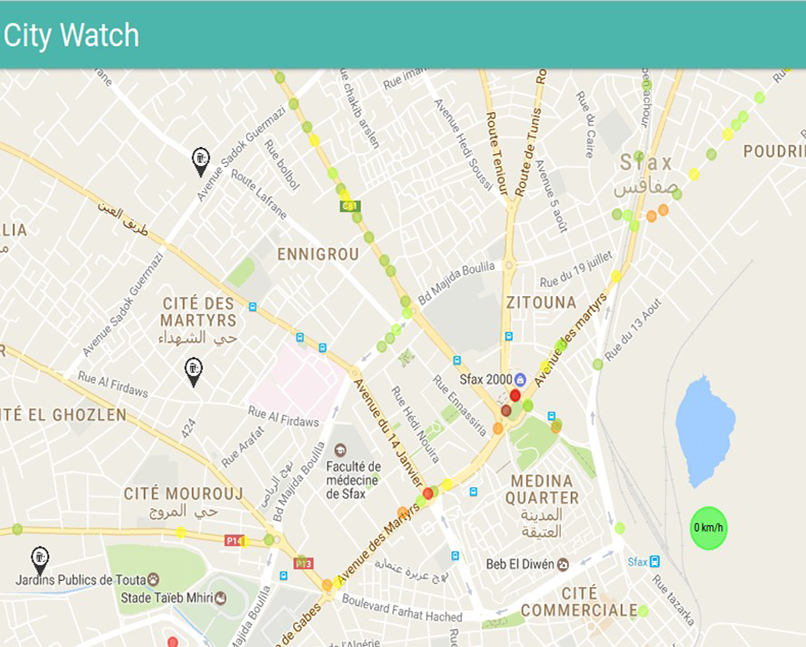
\includegraphics[width=.93\linewidth]{sprint2-dashboard-screenshot2}
  \caption{Groupement désactivé en zoom haut}
  \label{fig:sprint2-dashboard-screenshot2}
\end{subfigure}
\caption{Groupement des marqueurs des secousses en diffenet niveaux du zoom}
\end{figure}


\paragraph{"Application Mobile ``CityWatch''}
\TODO{App}
\subsubsection{Avis du ProductOwner}
\subsection{Travail contribué}
